

\documentclass[]{article}

\usepackage{indentfirst}
\usepackage{cmap}					% поиск в PDF
%\usepackage[T2A]{fontenc}			% кодировка
%\usepackage[utf8]{inputenc}			% кодировка исходного текста
\usepackage[english,russian]{babel}	% локализация и переносы
\usepackage{amsmath, amsfonts, amssymb, amsthm, mathtools}
\usepackage{icomma}
\usepackage{mathrsfs}
\usepackage{graphicx}
\usepackage{ upgreek }
\usepackage{array}
\usepackage{longtable}

%рисунки и все с ними связанное
\graphicspath{{pic/}}
\setlength\fboxsep{3pt}
\setlength\fboxrule{1pt}

\newcommand{\tyr}{Тырныауз }

\begin{document}
	
% НАЧАЛО ТИТУЛЬНОГО ЛИСТА
\begin{center}
	\hfill \break
	\large{Турклуб МГТУ им.Баумана}\\
	


\begin{figure}[h!]
	
	\centering{
\includegraphics[scale=0.3]{emblema}}

\end{figure}

	\hfill\break
	\hfill \break

	
	
	
	\large{Отчет о походе
		
		2 категории сложности
		
		совершенном с 25 июля по 9 августа 2020 года
		}\\
	\hfill \break
	\hfill \break
	\hfill \break
	
	\hfill \break
	
\end{center}

\hfill \break
\hfill \break

\normalsize{ 
	\begin{tabular}{ccc}
		
		
		Руководитель & \underline{\hspace{3cm}}& Волнухина Е.Д. \\\\
		
	
	\end{tabular}
}\\
\hfill \break
\hfill \break
\begin{center} Москва 2020 \end{center}
\thispagestyle{empty} % выключаем отображение номера для этой страницы
	
	
\section{Общие сведения о походе}
Основная идея похода была в том чтобы показать новичкам горы, и может, затащить их в турклуб. Изначально, в феврале, планировалась хорошая техничная горная двойка, но потом началась эпидемия, тренироваться в апреле и мае не вышло. Бонусом отстрелилось несколько опытных участников, поэтому техничность пришлось сокращать. Вот так и получилось что из 5 шт 1Б осталось только 2 шт, да и те руковод ходил в 2017 году.

В целом поход можно разбить на три логические части: занятия, часть 1 к.с. и часть 2 к.с. Так было сделано по нескольким причинам:

1. Поскольку участникам не хватало опыта, МКК поставило условие перед частью 2к.с. сделать часть 1 к.с. с проходом через населенку откуда можно слить разочаровавшихся туристов.

2. Так как, опять же, много новичков, велика вероятность внезапных приключений с горняшкой, собственным ощущением себя в походе и все такое. Поэтому народ постепенно привыкал к новым условиям не на маршруте, а на занятиях недалеко от а/л. Что, кстати, сыграло хорушую роль, поскольку на второй день занятий у одного участника развалились (вот прям совсем) ботинки.

Пропуска основная часть команды получила по почте, два человека забирали у водителя. Никаких сложностей с этим не было, хотя пару человек жаловалось что пограничники ругались на качество фотографии паспорта.

В район забрасывались на самолете, а затем и на автобусе. Один участник опоздал на самолет до Минвод, поэтому прилетел в Беслан пару часов спустя, откуда на такси за 3600 доехал до поворота на Адылсу, где через 7 минут встретил группу.

Автобус туда заказывали у Бориса Сорокуева, на 11 человек это стоило 14000. Обратно добирались маленькими группами самостоятельно, поскольку все уезжали в разное время.

 
\subsection{Участники похода}
Всего в поход пошло 11 человек, 4 женщины и 7 мужчин. Благодаря такому соотношению вес общественного снаряжения и еды на девочек рассчитывался с коэффициентом 0.7.
	
	\begin{center}
		\begin{longtable}{|m{0.3cm}|m{3cm}|m{0.7cm}|m{1cm}|m{2cm}|m{4cm}|}
		\caption{\label{tab: people} Данные об участниках}\\
			\hline
			№ & Имя & г.р.& Опыт & должность & Фото  \\	\hline
			1 & Волнухина Елена Дмитриевна&1998&1ГР, 2ГУ, нк.с эл.4ГУ&руководитель, завснар&
			   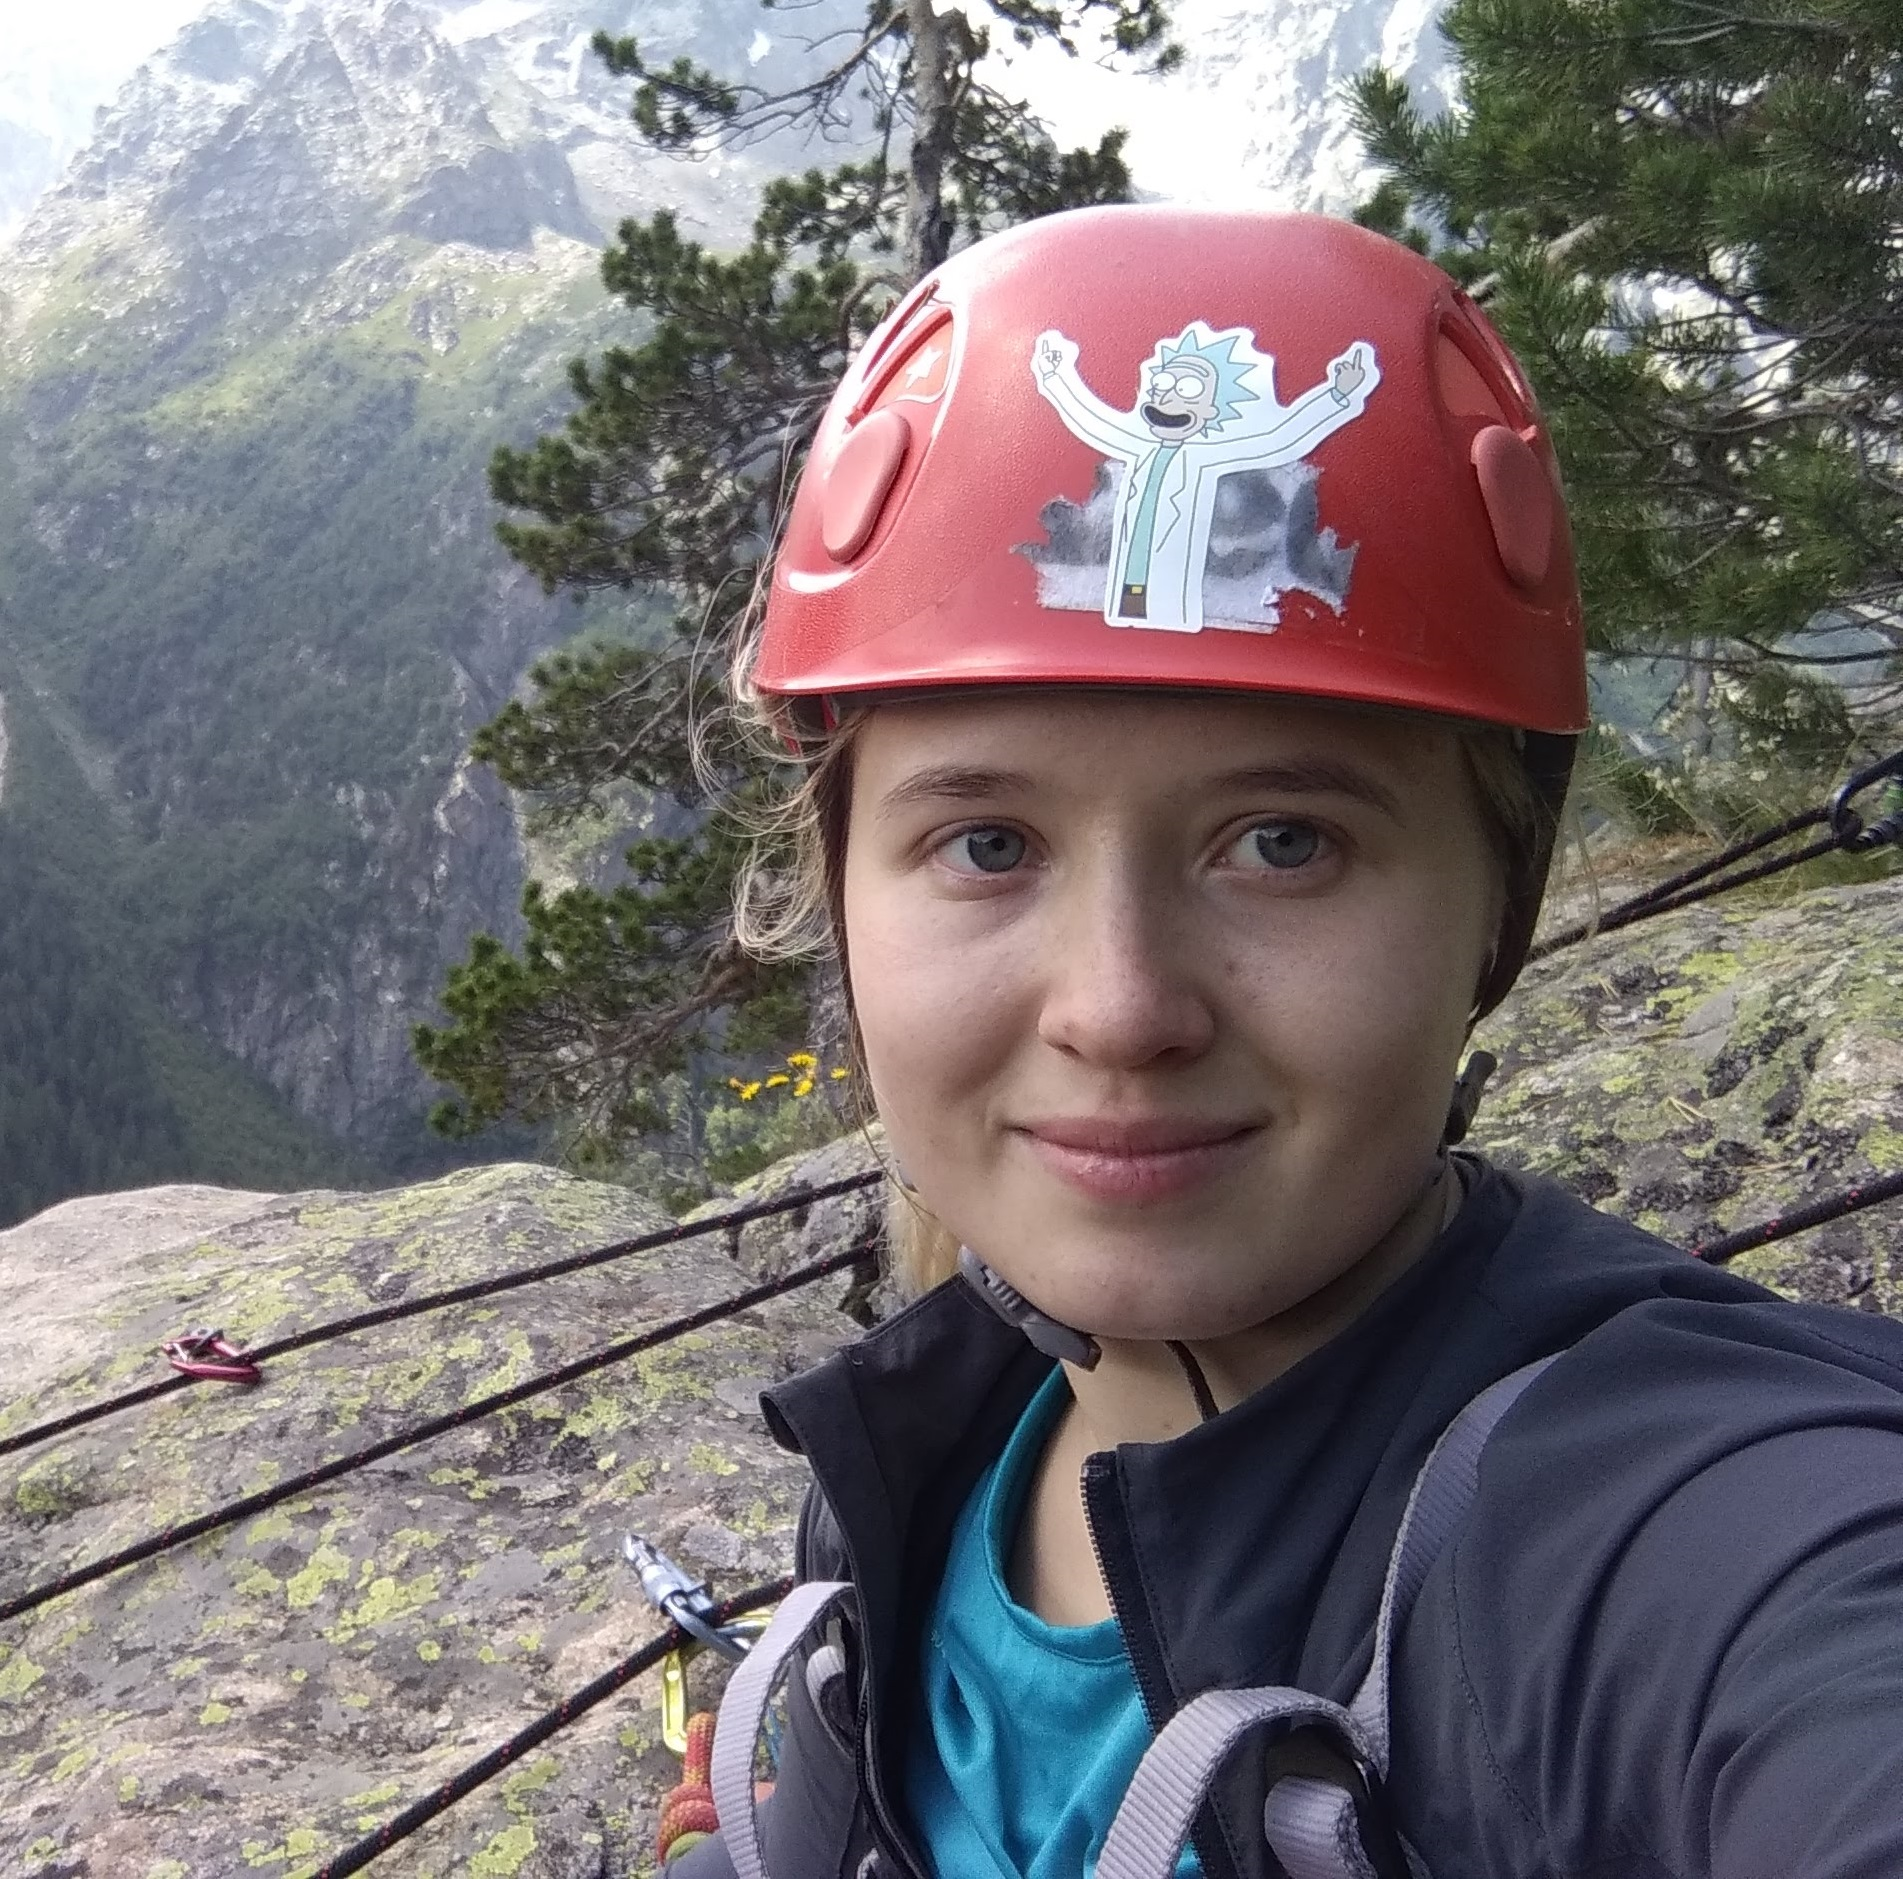
\includegraphics[width=4cm]{Lena}\\
			\hline
			
			2 &Чаплыгин Алексей Владимирович&1987&5ГУ, нк.с эл.4ГР&инструктор-гид&
			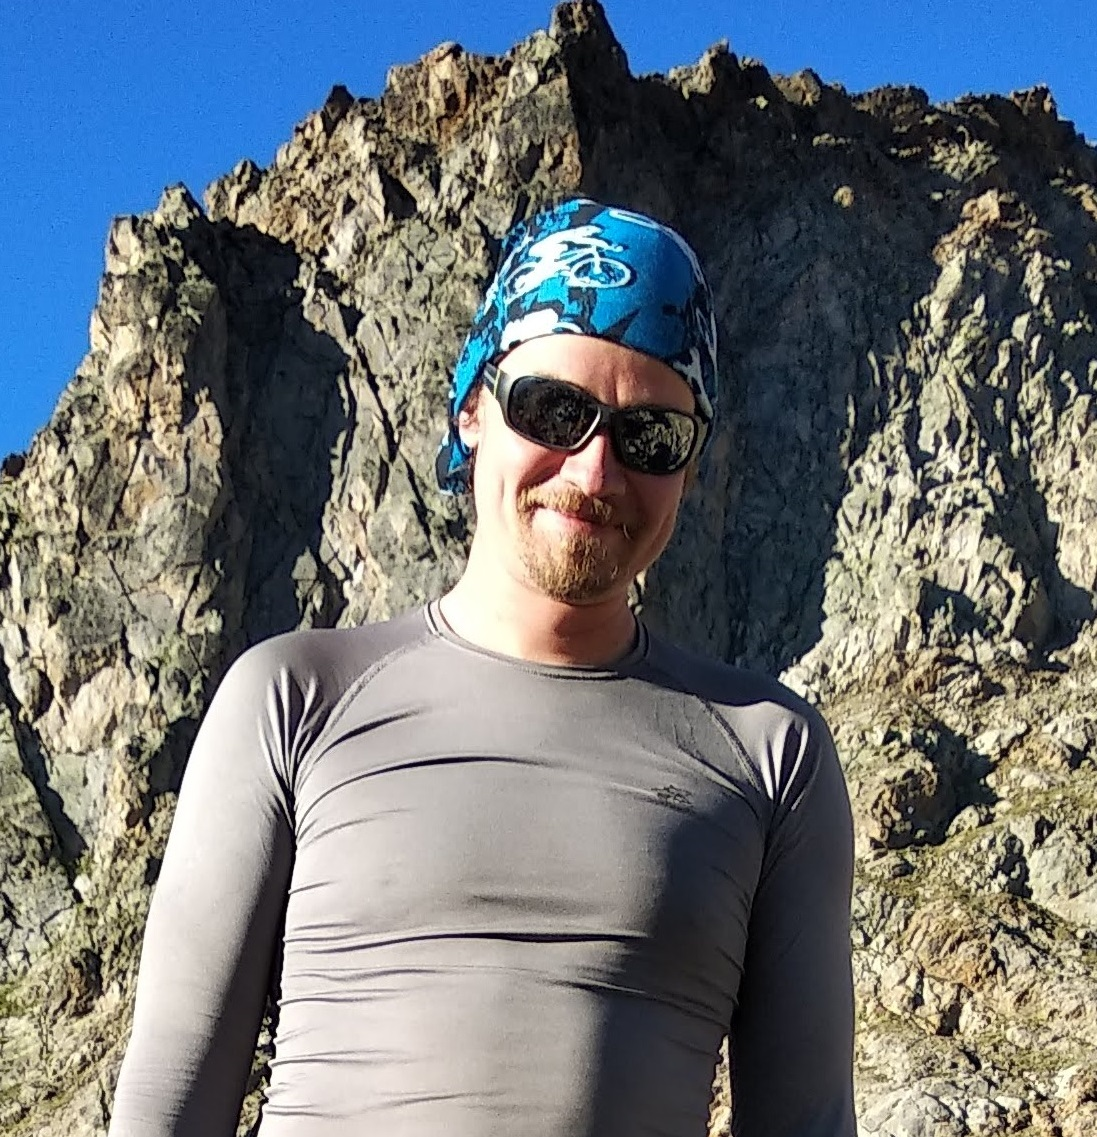
\includegraphics[width=4cm]{Chapa}\\
			\hline
			3 &Фомин Антон Андреевич&1992&ПВД&завхоз&
			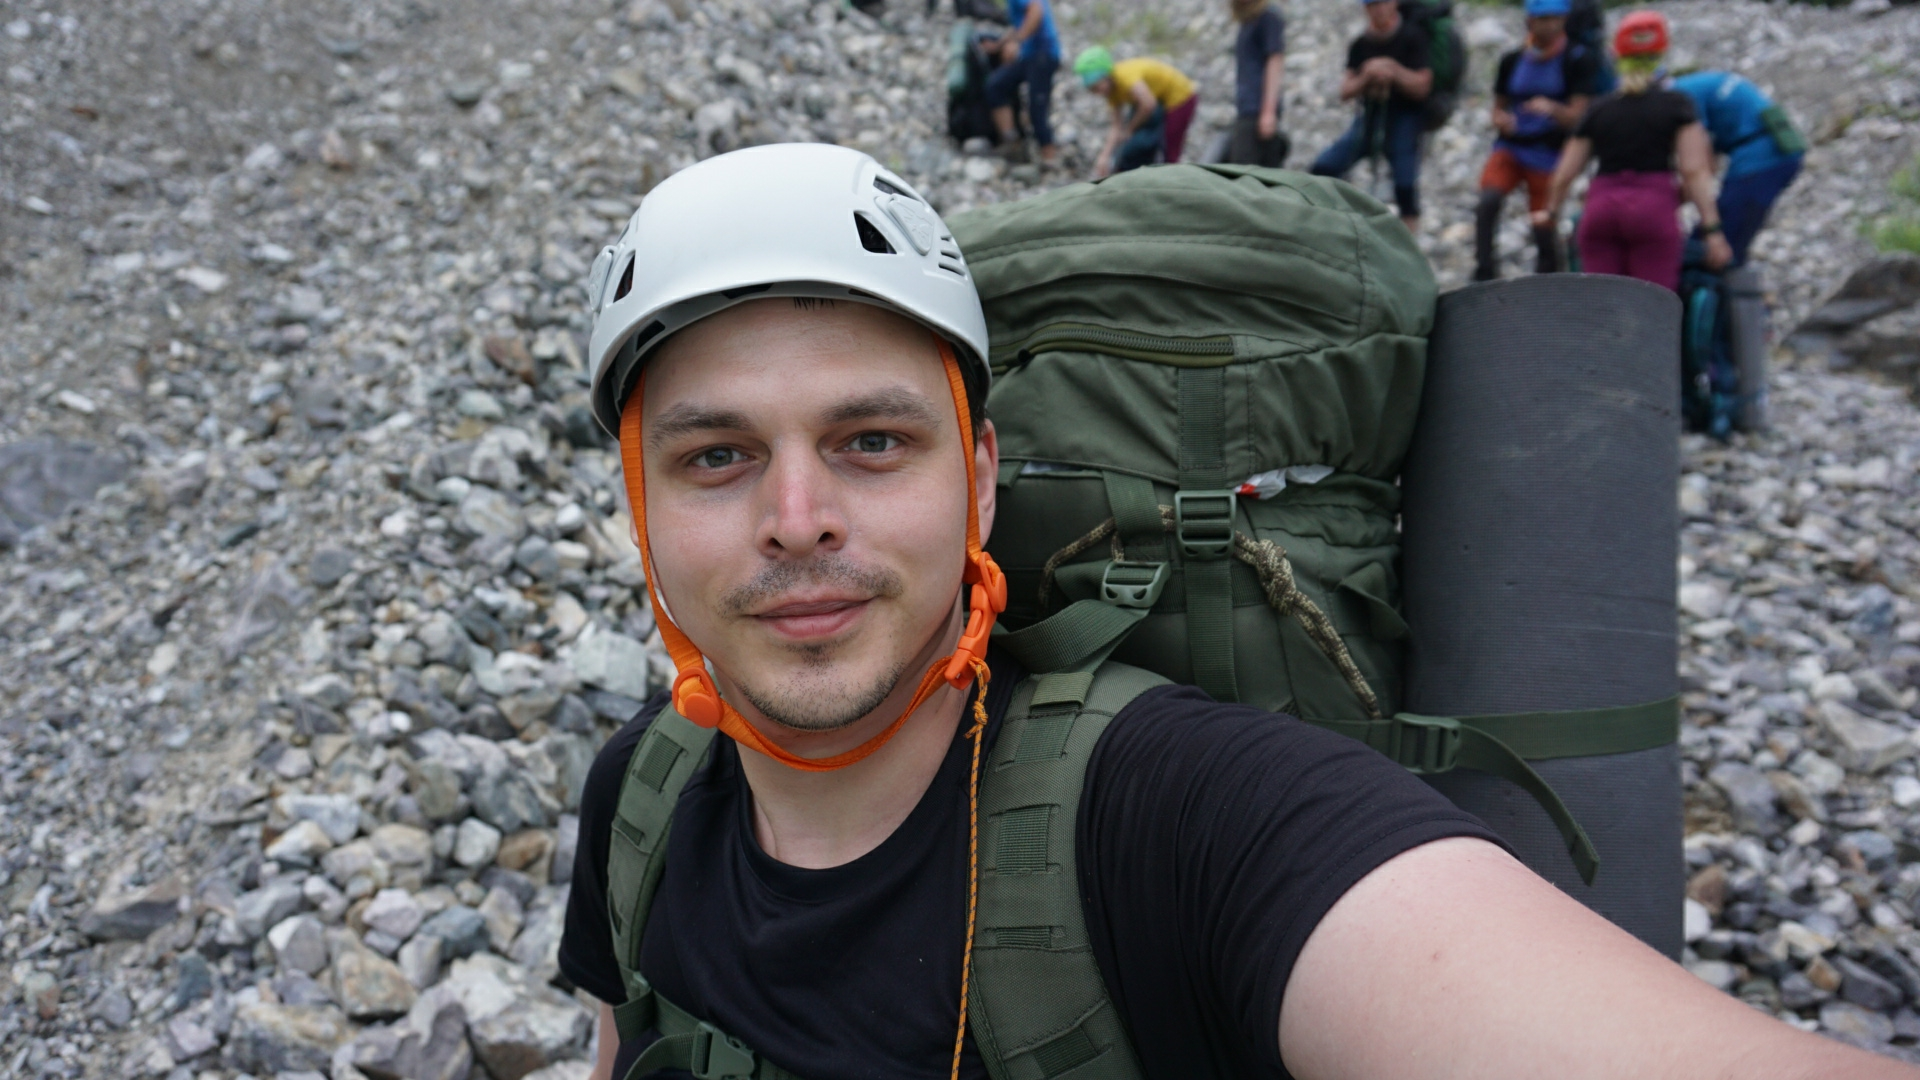
\includegraphics[width=4cm]{Anton_F}\\
			\hline
			4 &Дудякова Галина Леонидовна&1990&1ПР&&
			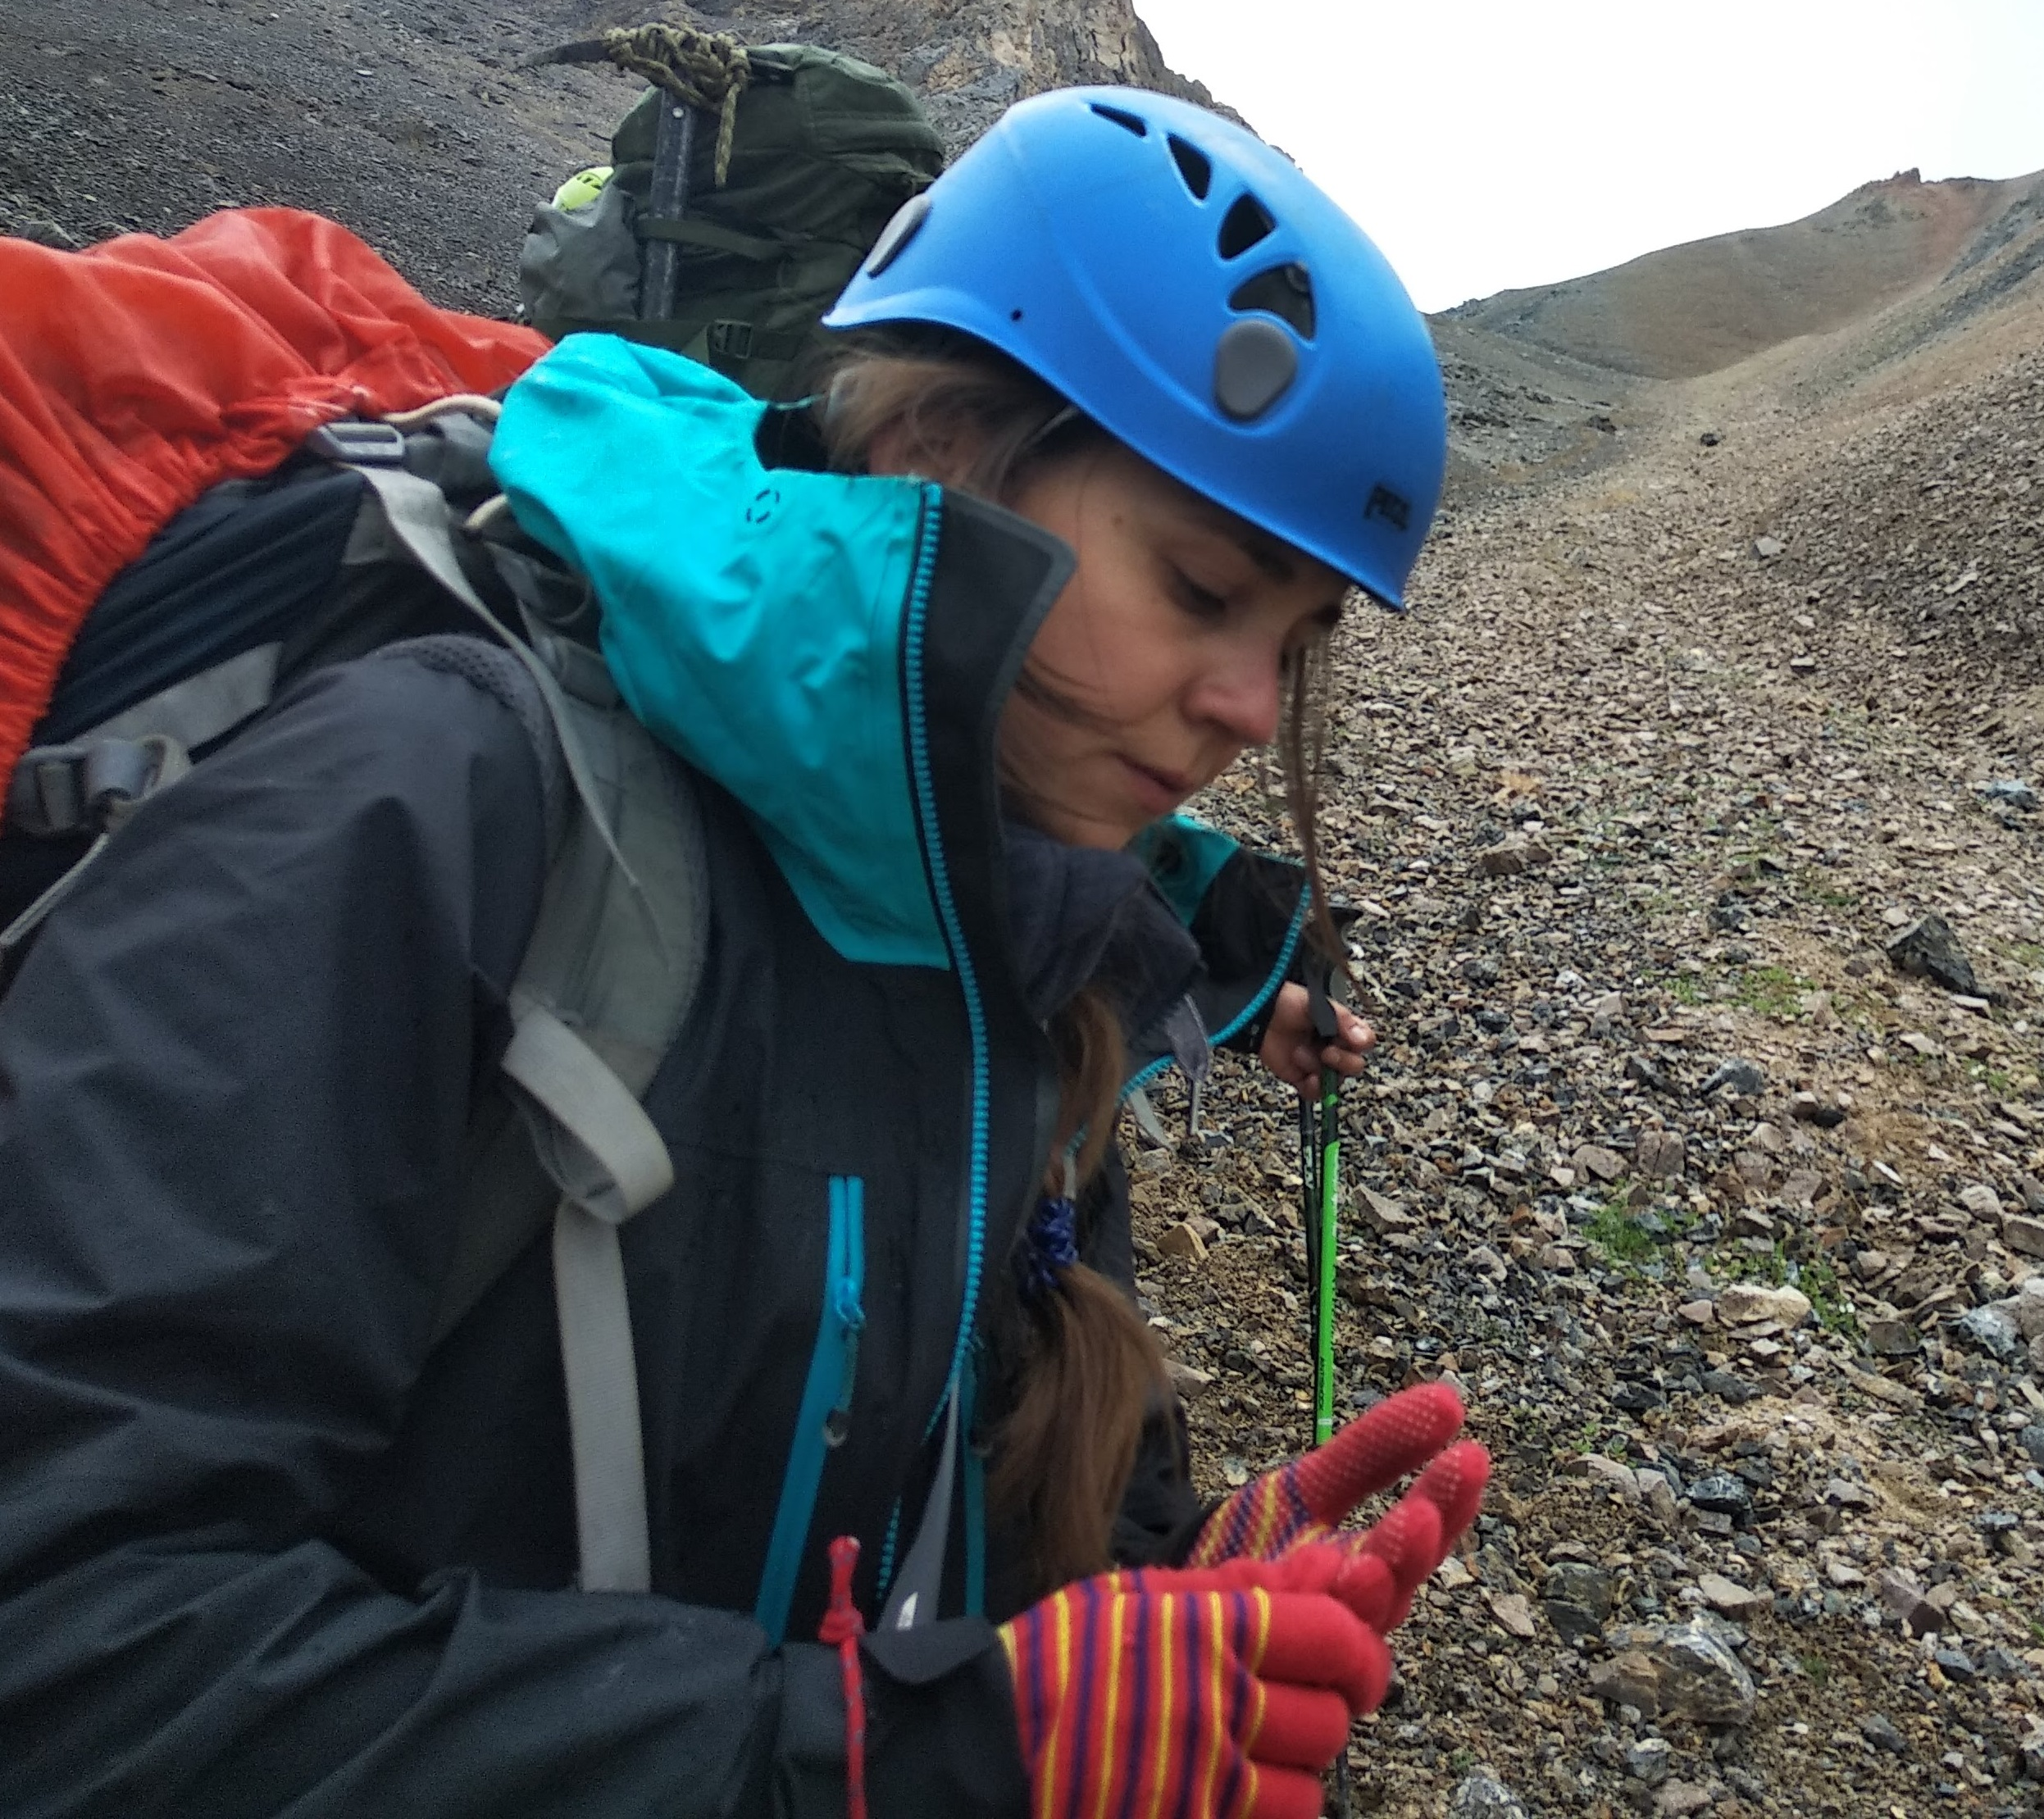
\includegraphics[width=4cm]{Gala}\\
			\hline
			5 &Мухаметшин Максим Ильгамович&1998&ПВД&Тех.писатель&
			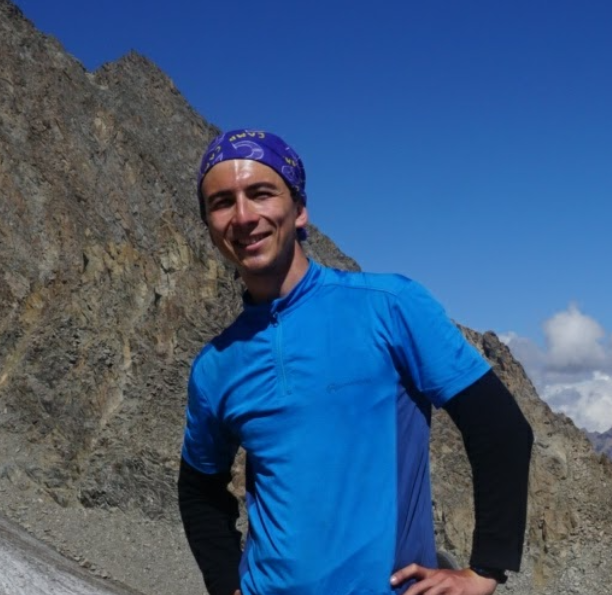
\includegraphics[width=4cm]{Max_M}\\
			\hline
			6 &Галкин Александр Васильевич&1994&ПВД&Лир.писатель&
			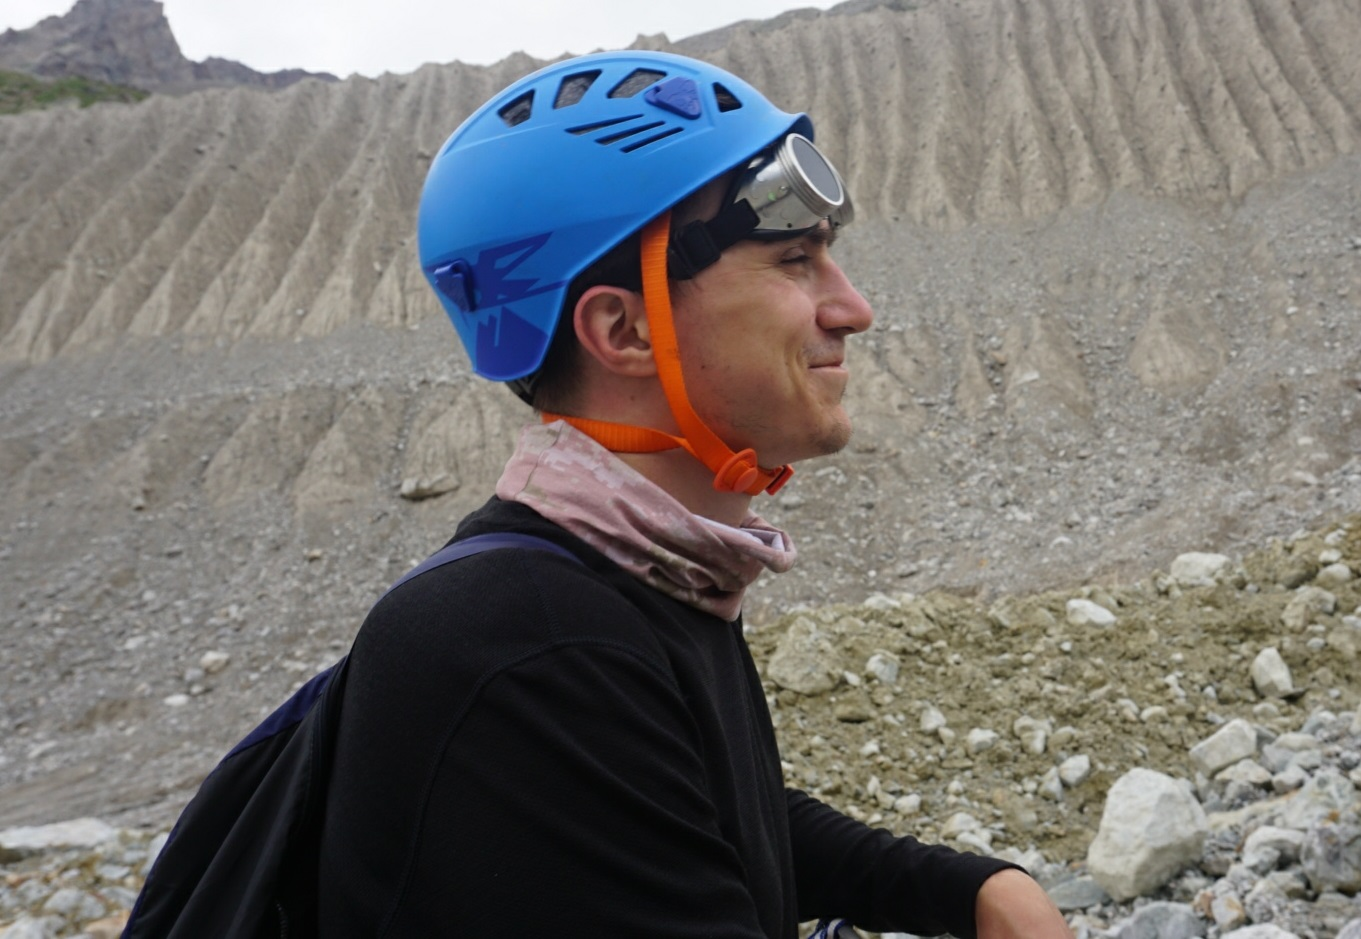
\includegraphics[width=4cm]{Alex}\\
			\hline
			
			
			7 &Лебедева Вера Владимировна&2001&ПВД&Эколог&
			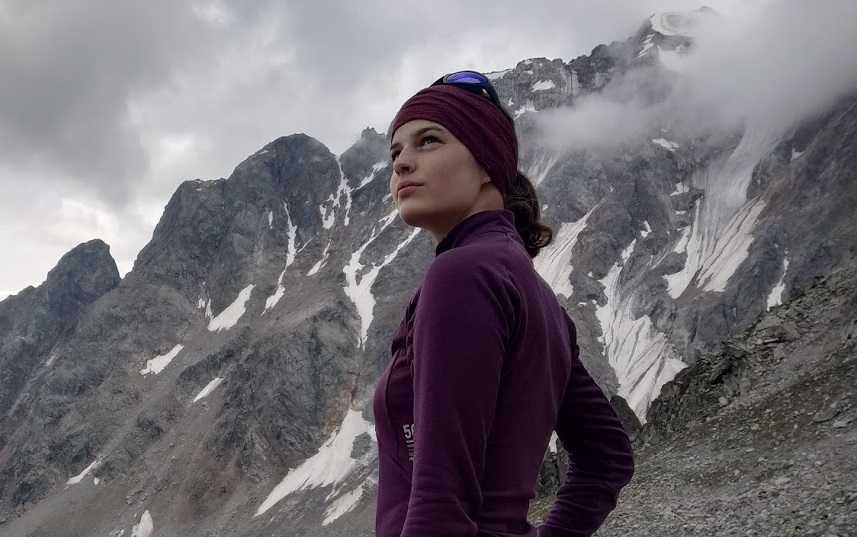
\includegraphics[width=4cm]{Vera}\\
			\hline
			8 &Картушина Кристина Леонидовна&1993&ПВД&Фотограф&
			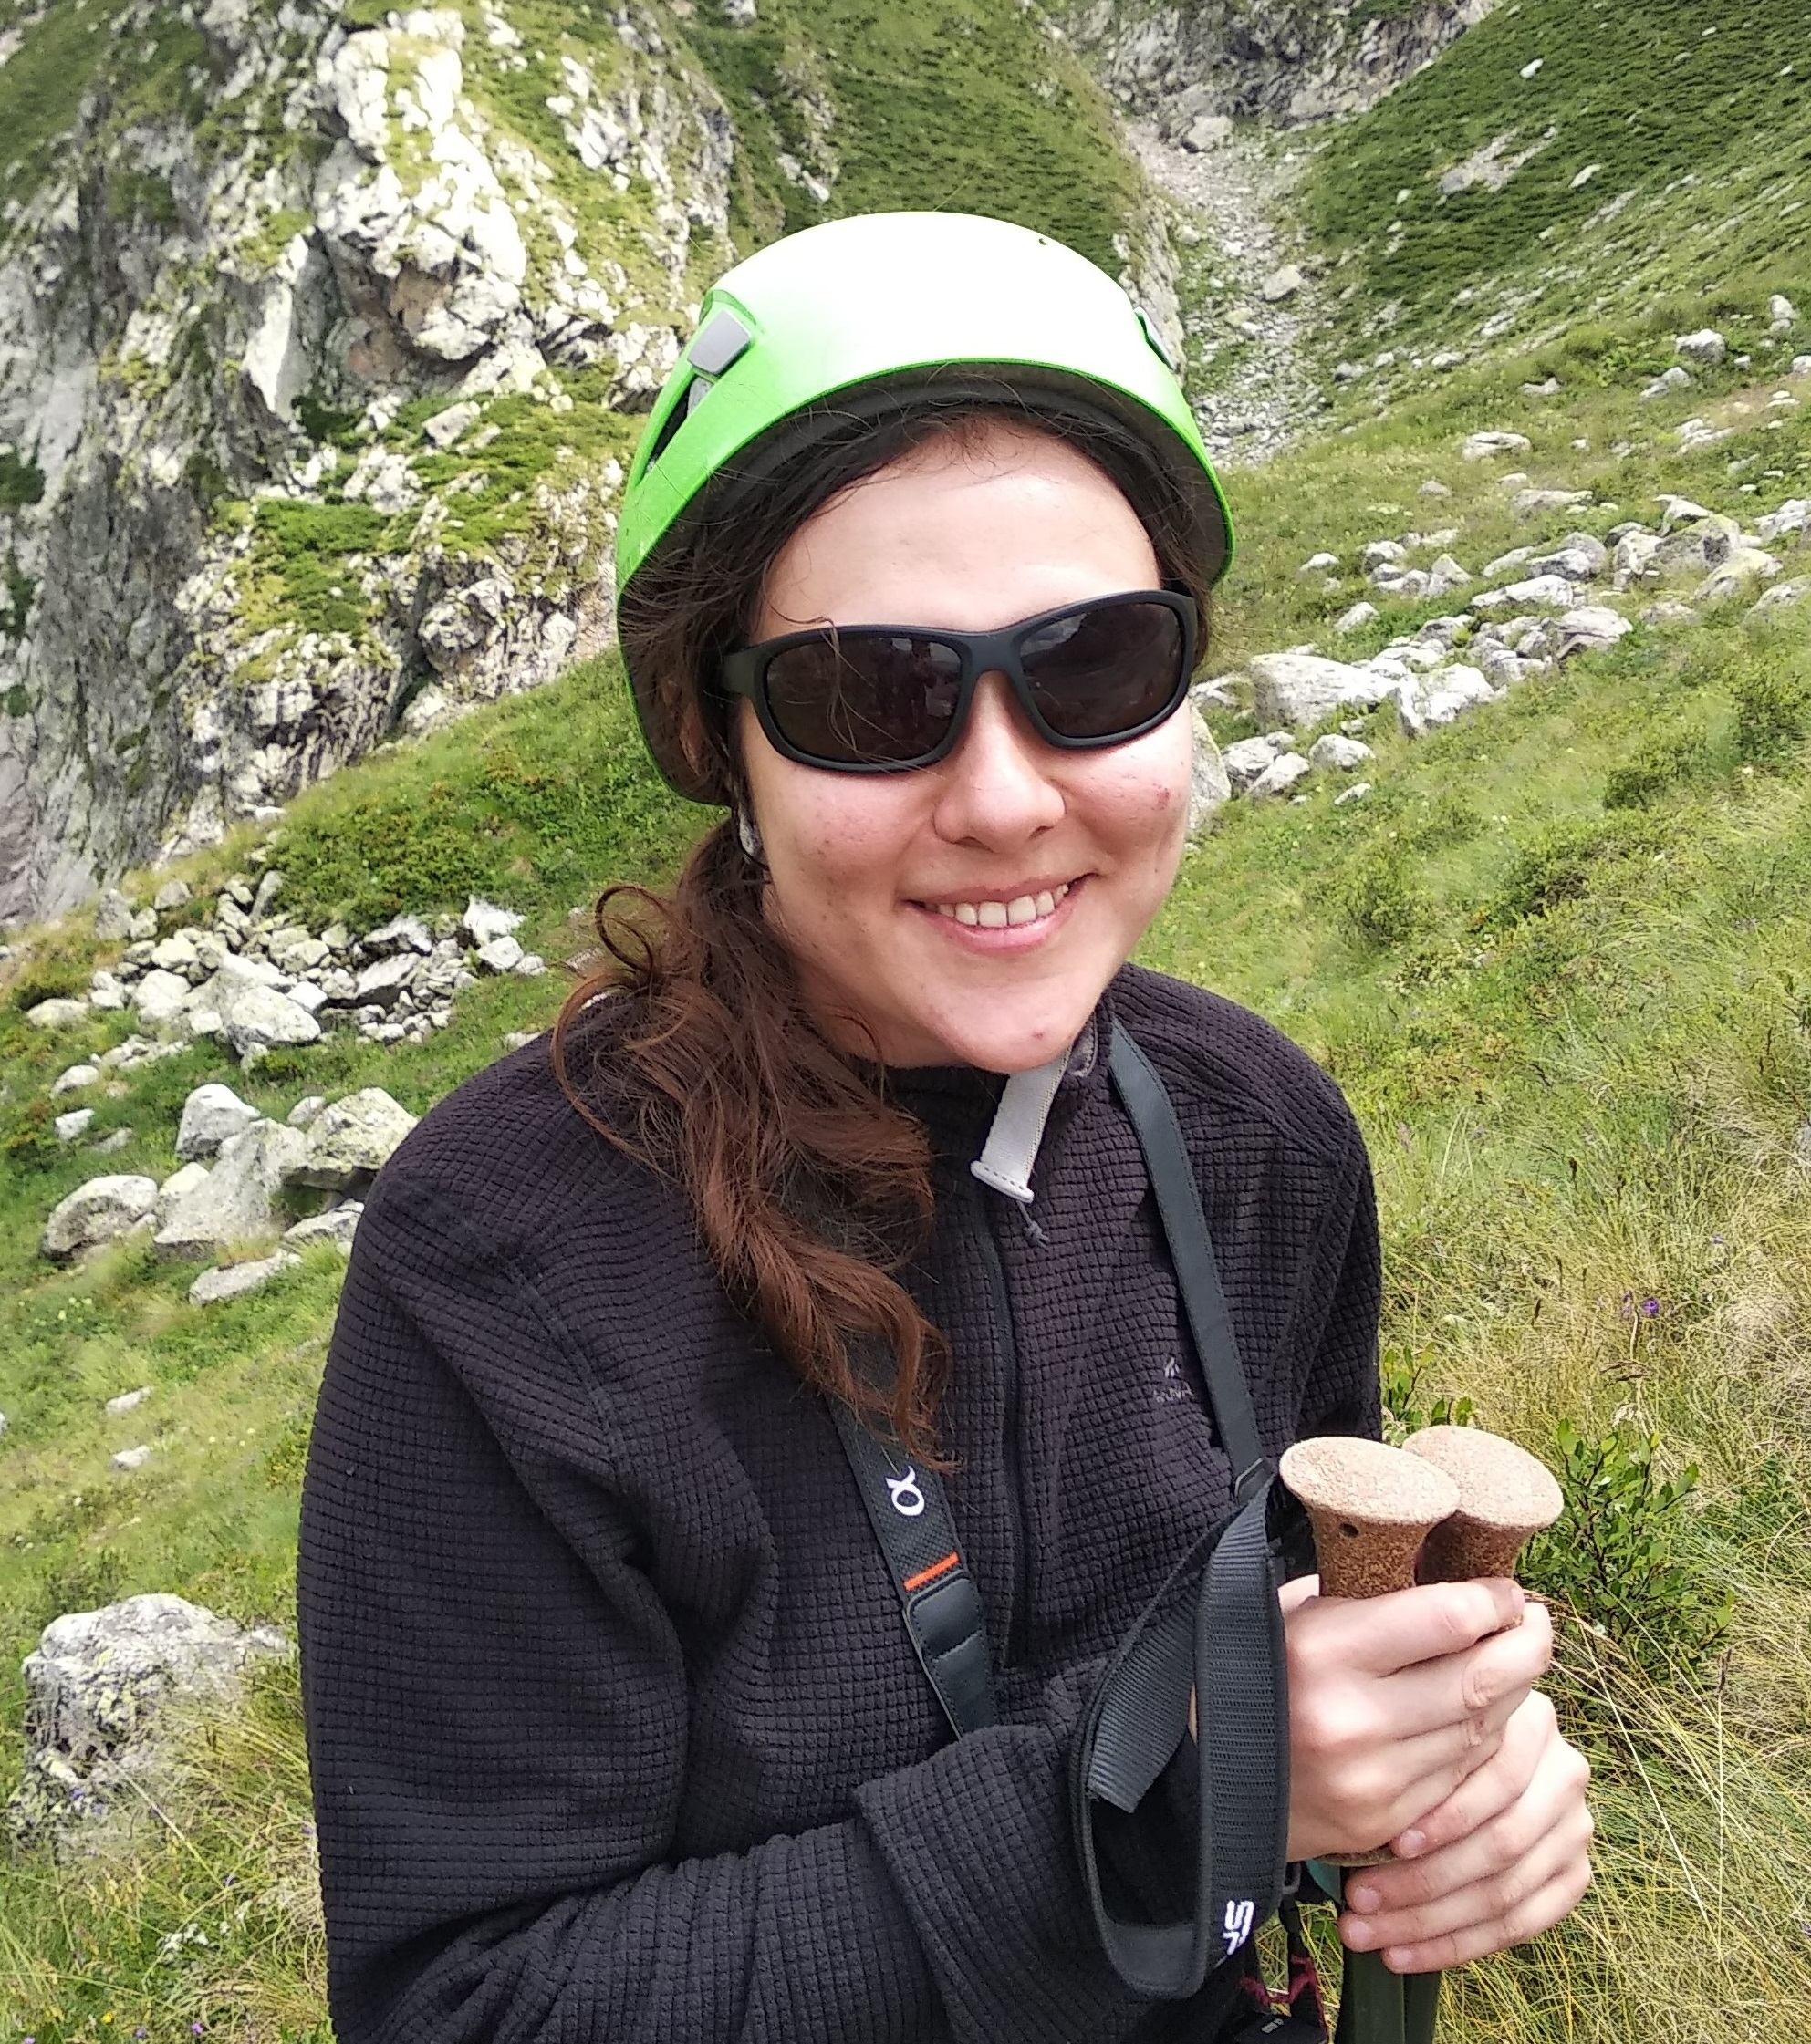
\includegraphics[width=4cm]{Kris}\\
			\hline
			9 &Синицин Антон Андреевич&1999&ПВД&Логист&
			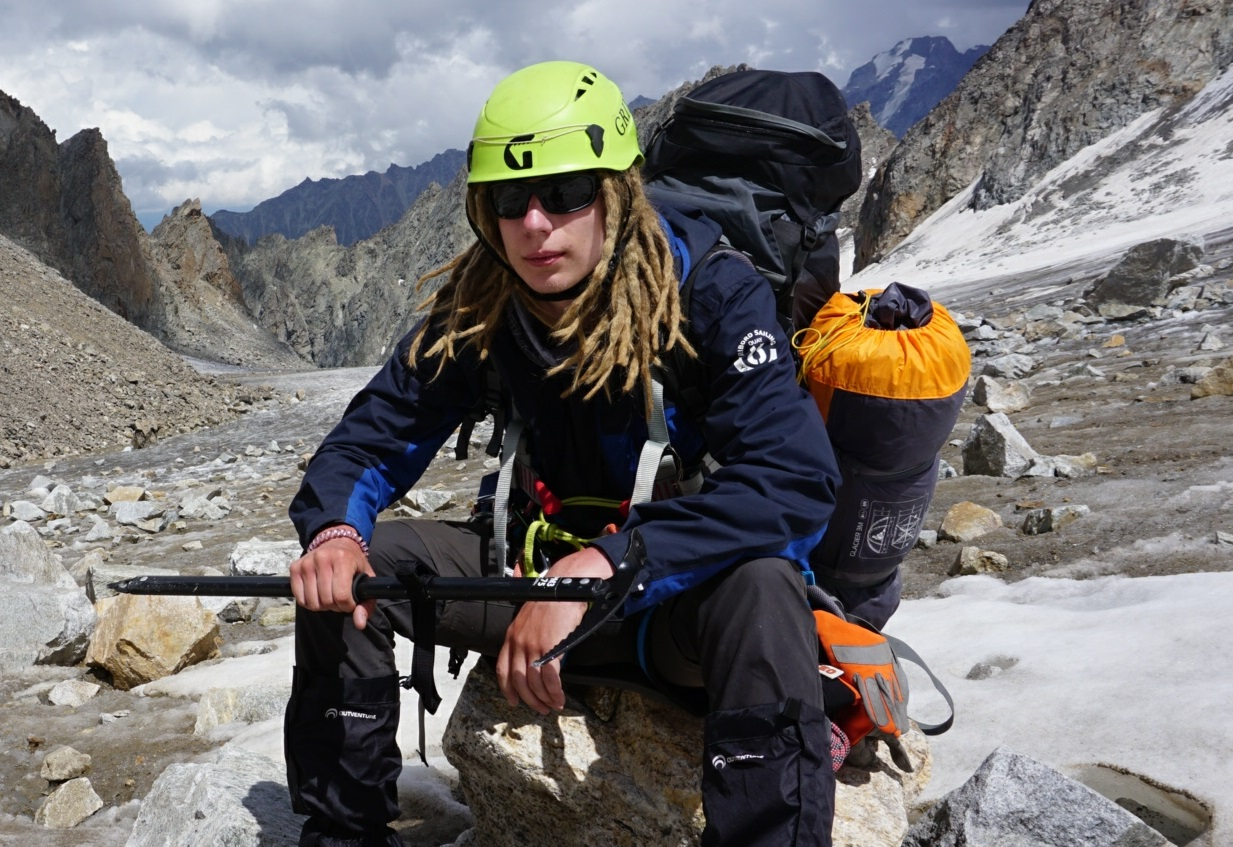
\includegraphics[width=4cm]{Anton_S}\\
			\hline
			10 &Байбеков Кирилл Сергеевич&1992&1ГУ&Медик&
			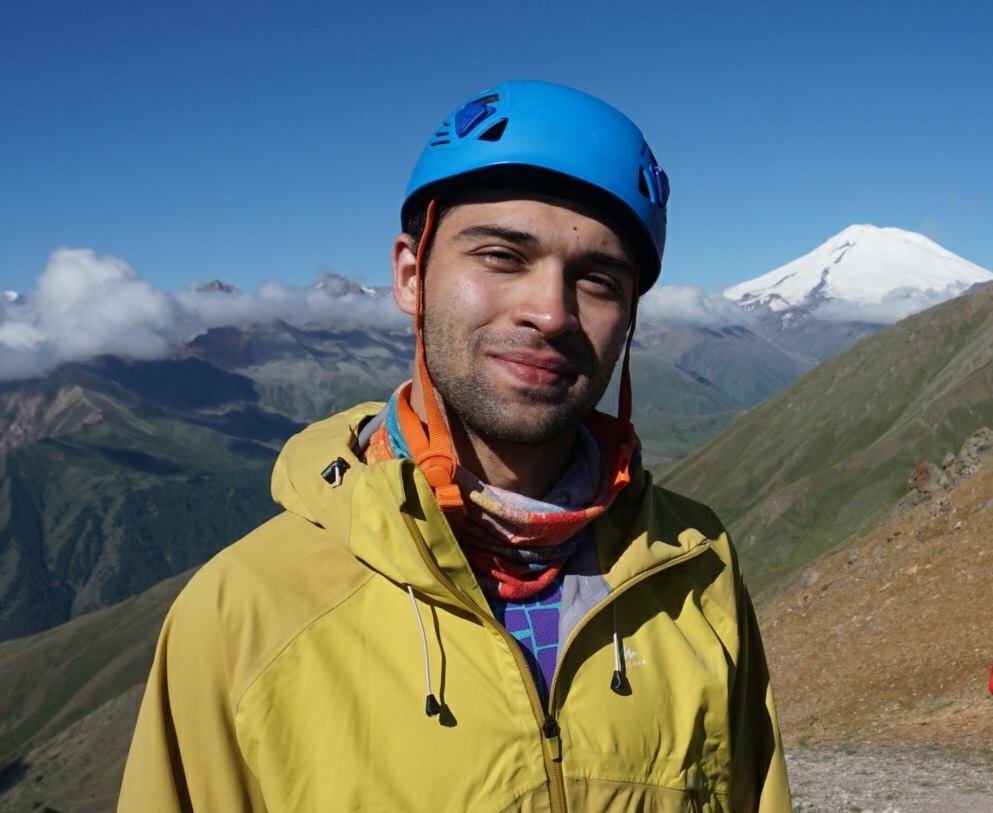
\includegraphics[width=4cm]{Kiril}\\
			\hline
			11 &Семёнов Максим Николаевич&1991&1ПУ&Реммастер&
			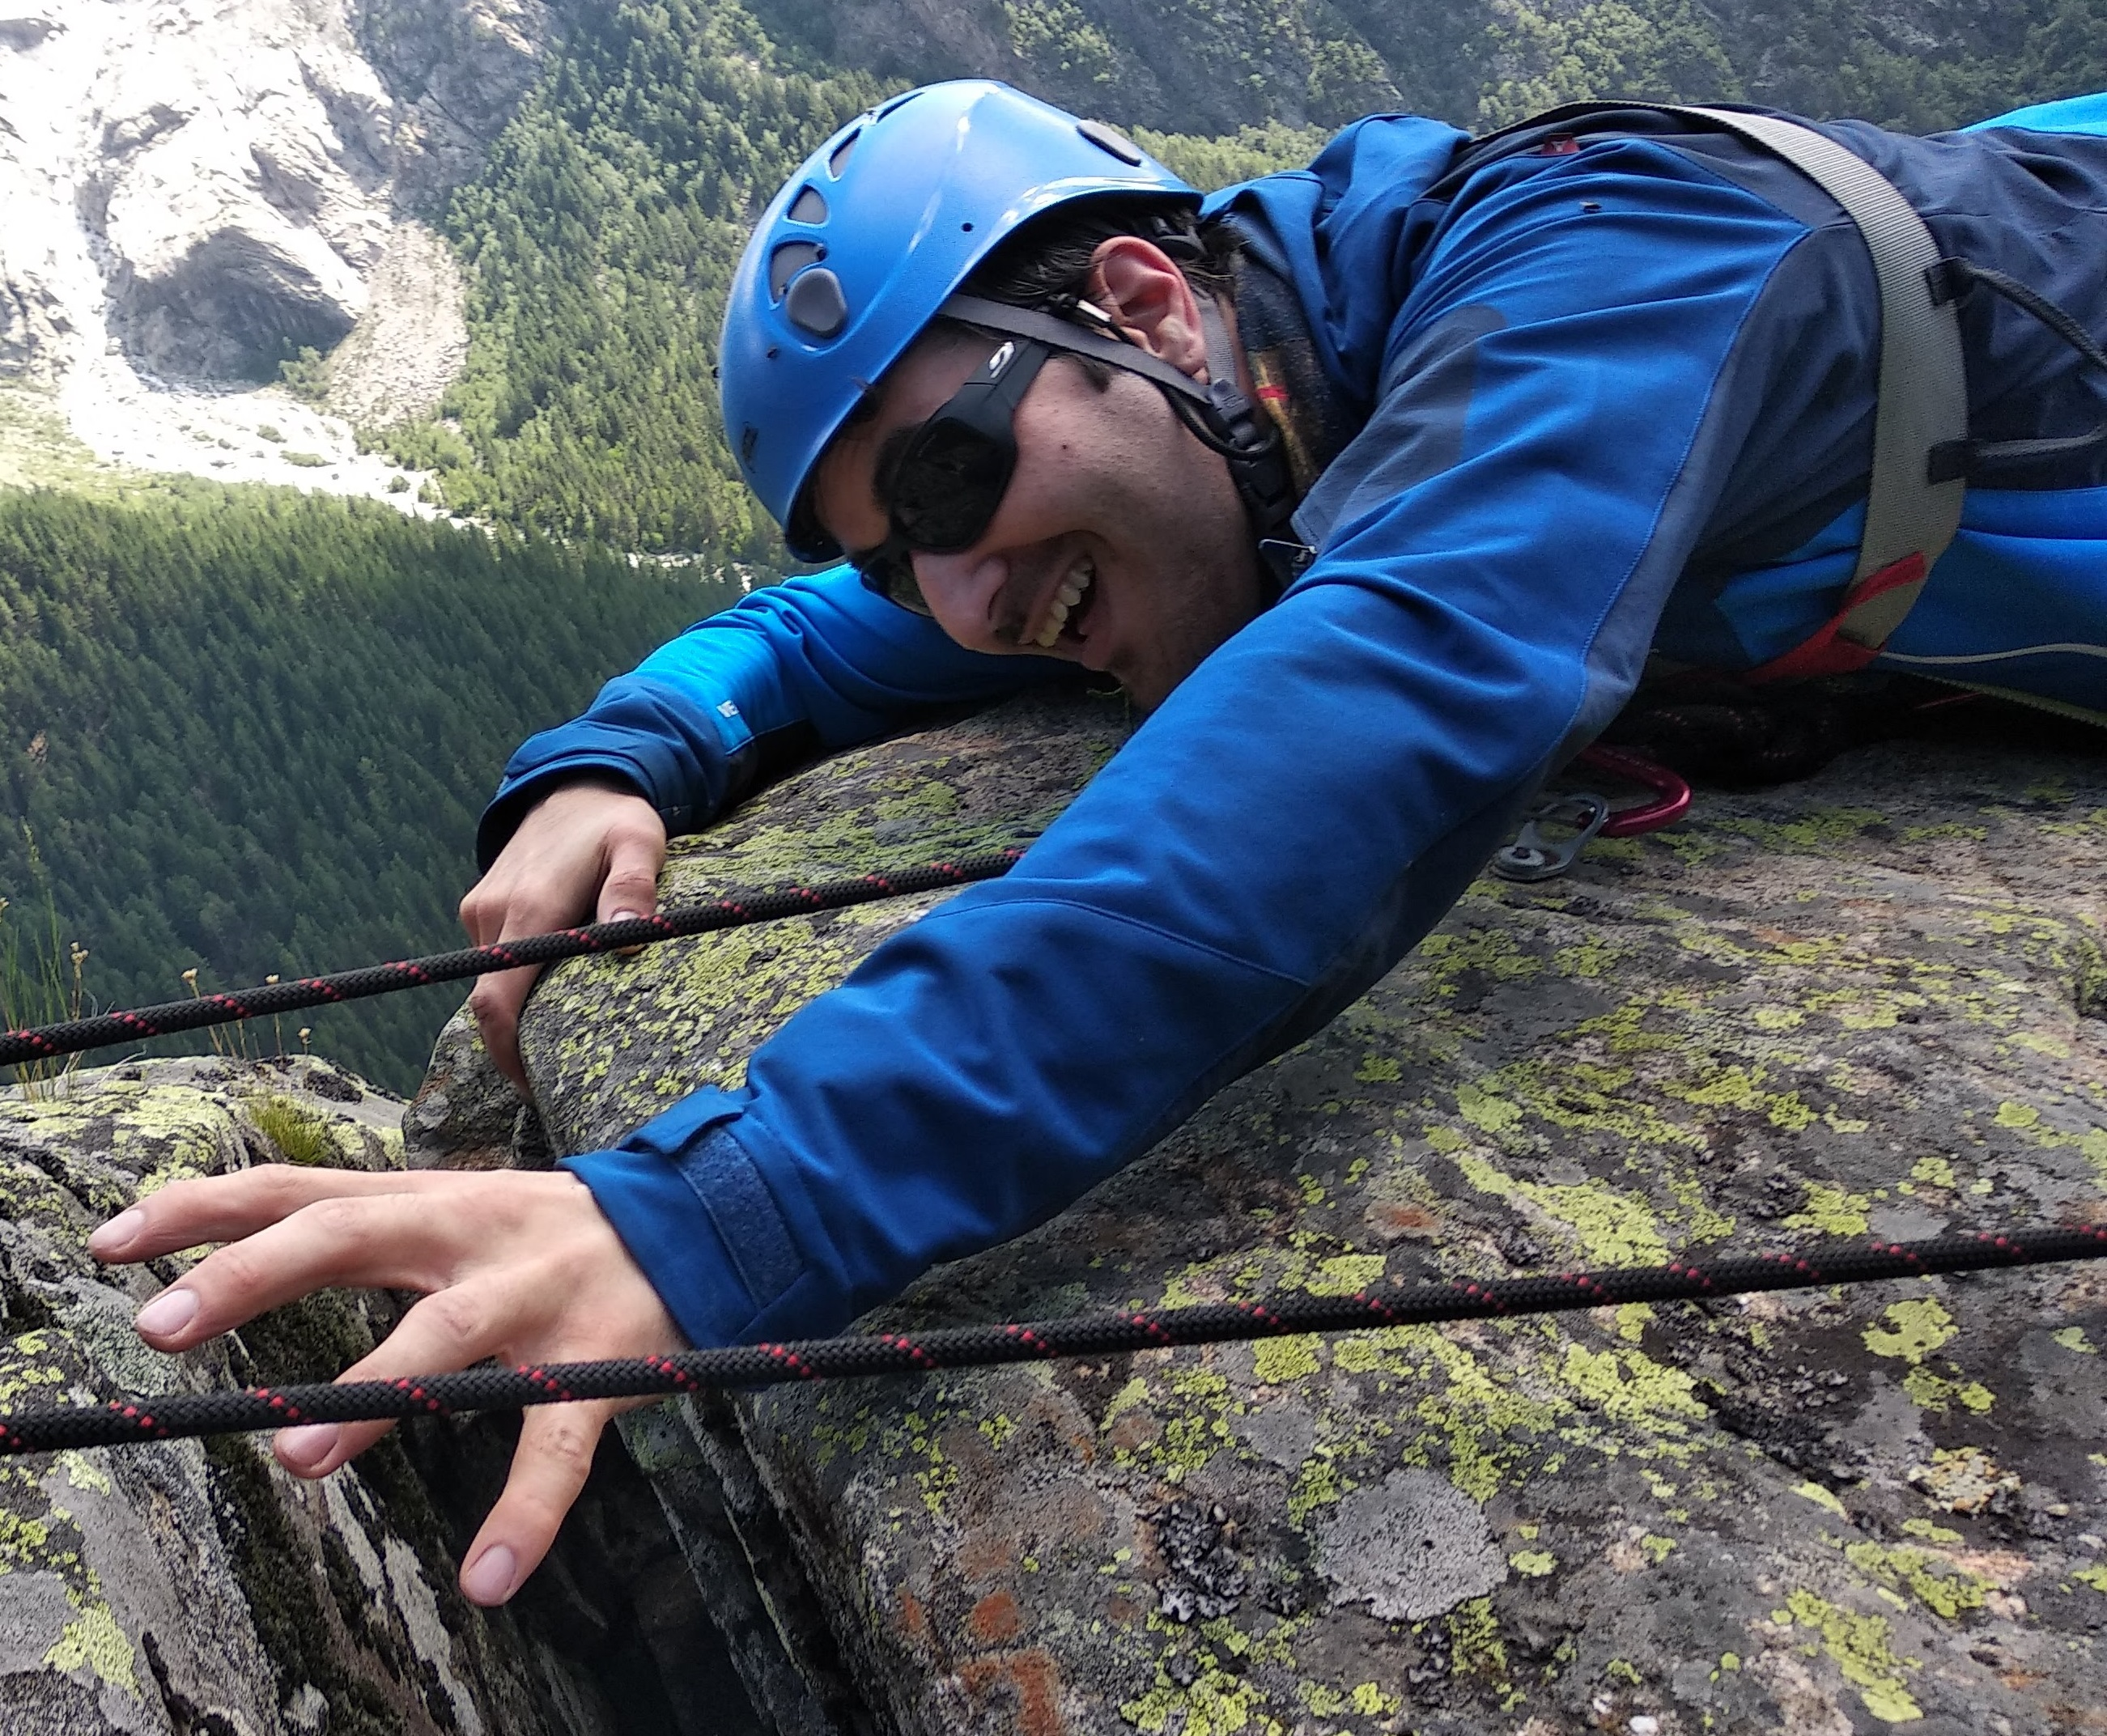
\includegraphics[width=4cm]{Max_S}\\
			\hline
			12 &Месснер&хз&ПВД&расходный участник&
			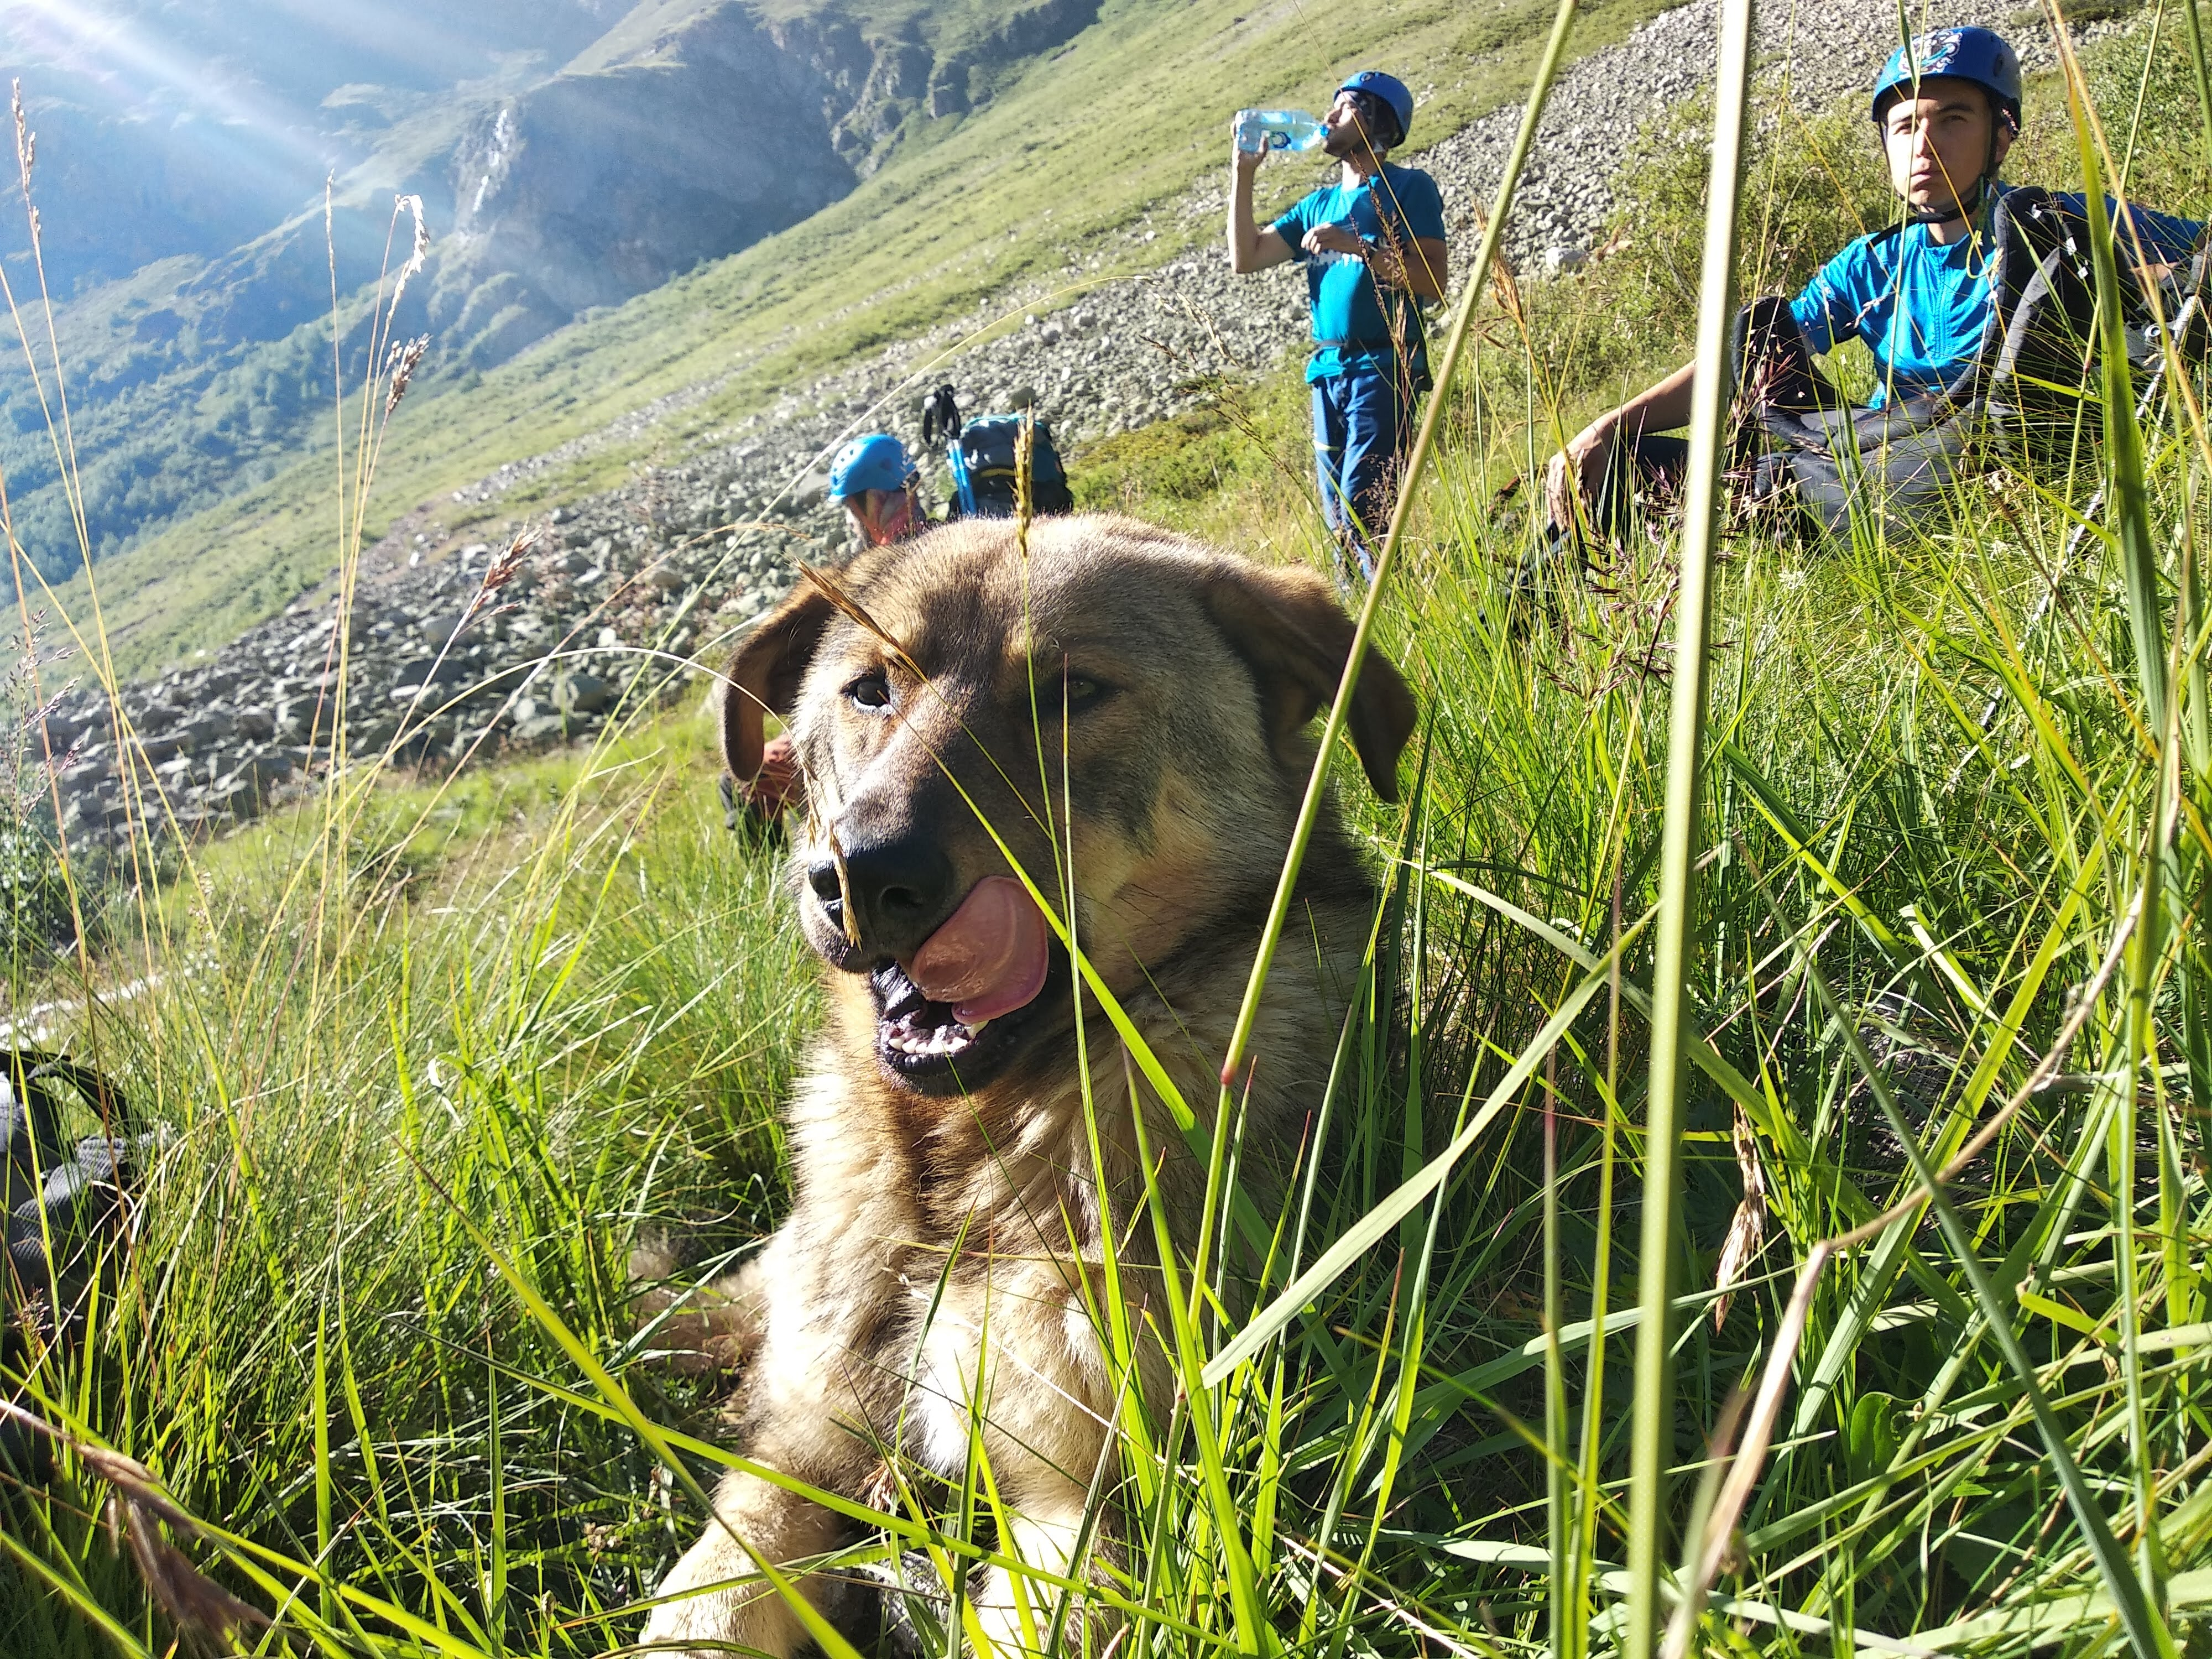
\includegraphics[width=4cm]{Messner}\\
			\hline			
		\end{longtable}
	\end{center}



\subsection{Маршрут}

\textbf{Планируемая нитка маршрута}
а/л Джантуган-л.Джанкуат-а/лДжантуган-л.Кашкаташ-а/л Джантуган- пос.Тырныауз- д.р. Тырныауз-пер.Тырныауз (1А,3400)-пер. Суарык (1А, 3200)- д.р.Зугулла-д.р.Кыртык-пос.Верхний Баксан-д.р. Адырсу- база МЧС- д.р.Джаловчат- пер.Джаловчат(1Б, 3666)- пер.Курмычи(1Б, 3801)-в.Узловая(1А, 3970)-в.Курмычи (1Б, 4045)-пер.ВЦСПС (1Б, 3693)-а/л Джантуган- д.р.Адылсу-пос.Эльбрус- д.р. Ирикчат- пер.Терсколак (1Б, 3527)- д.р.Терскол- пос.Терскол


\textbf{Фактическая нитка маршрута}

а/л Джантуган-л.Джанкуат-а/л Джантуган-л.Кашкаташ-а/л Джантуган- пос.Тырныауз- д.р. Тырныауз-пер.Тырныауз (1А,3400)-пер. Суарык (1А, 3200)- д.р.Зугулла-д.р.Кыртык-пос.Верхний Баксан-д.р. Адырсу- база МЧС- д.р.Джаловчат- пер.Джаловчат(1Б, 3666)- пер.Курмычи(1Б, 3801)-а/л Джантуган- д.р.Адылсу-пос.Эльбрус- д.р. Ирикчат-  пер.Терсколак (1Б, 3527)- д.р.Терскол- пос.Терскол

\textbf{Причины изменения}
Было решено отказаться от траверса пер.Курмычи-пер.ВЦСПС поскольку за ночь до этого группа пурговала и вымоталась, также несколько участников чувствовали себя не очень хорошо из-за горной болезни.
В итоге группа воспользовалась запасным вариантом пути.

График движения группы представлен в таблице \ref{tab:grafik}. Длина пути указана без учета коэффициента 1.2.

\begin{table}[h!]
	\caption{\label{tab:grafik} График движения фактический}
	\begin{center}
		\begin{tabular}{|p{0.7cm}|p{0.3cm}|p{5cm}|p{0.9cm}|p{1cm}|p{1cm}|}
			\hline
			Дата&№& Участок пути & Набор/ сброс, м & Длина пути, км & ЧХВ, ч.м.\\ \hline
			25.07&-2&а/л Джантуган- скальная лаборатория- а/л Джантуган&+320 -320 & 3.2 & 2.0\\ \hline
			26.07&-1&а/л Джантуган-л.Джанкуат- а/л Джантуган&+700 -700 & 12 & 6.0\\ \hline
			27.07&0&а/л Джантуган- тропа на л.Кашкаташ- а/л Джантуган&+530 -530 & 3.8 & 4.40\\ \hline
			28.07&1&а/л Джантуган- переезд- п.Тырныауз- д.р. Тырныауз&+1800 -430 & 19 & 6.10\\ \hline
			29.07&2&д.р.Тырныауз- \textbf{пер.Тырныауз (1А, 3400)}- д.р.Суарык &+600 -340 & 4.5 & 3.0\\ \hline
			30.07&3&д.р. Суарык-\textbf{пер.Суарык (1А, 3200)}- д.р.Зугулла-пос. Верхний Баксан-д.р.Адырсу &+800 -2100 & 18 & 6.50\\ \hline
			31.07&4&д.р. Адырсу-д.р.Джаловчат &+1500 -0 & 12 & 4.0\\ \hline
			1.08&5&д.р.Джаловчат- \textbf{пер.Джаловчат(1Б,3570)}- подход под пер. \textbf{пер. Курмычи (1Б,3740)} &+730 -80 & 4.4 & 4.50\\ \hline
			2.08&6&отсидка &0 & 0 & 0\\ \hline
			3.08&7&пер. \textbf{пер.Курмычи (1Б, 3740)} - д.р. Адылсу - а/л Джантуган &+160 -1630 & 7 & 3.30\\ \hline
			4.08&8& а/л Джантуган- пос.Эльбрус- д.р.Ирик &+740 -670 & 16 & 2.30\\ \hline
			5.08&9& д.р.Ирик- пер. \textbf{пер. Терсколак (1Б, 3600)}-ночевки под Терсколаком  &+1200 -330 & 9.5 & 5.30\\ \hline
			6.08&10& д.р.Терскол -пос.Терскол  &+000   -1000 & 5.8 & 2.20\\ \hline
			\multicolumn{6}{|c|}{Итого} \\ \hline
			&&&	+9080 -8130 &	115.2&		 \\ \hline	
			
		\end{tabular}
	\end{center}
\end{table}
С учетом коэффициента 1.2 было пройдено 138 км.
Схема итогового пути на рис.\ref{map_all}.
\begin{figure}[h!] 
	
	\centering{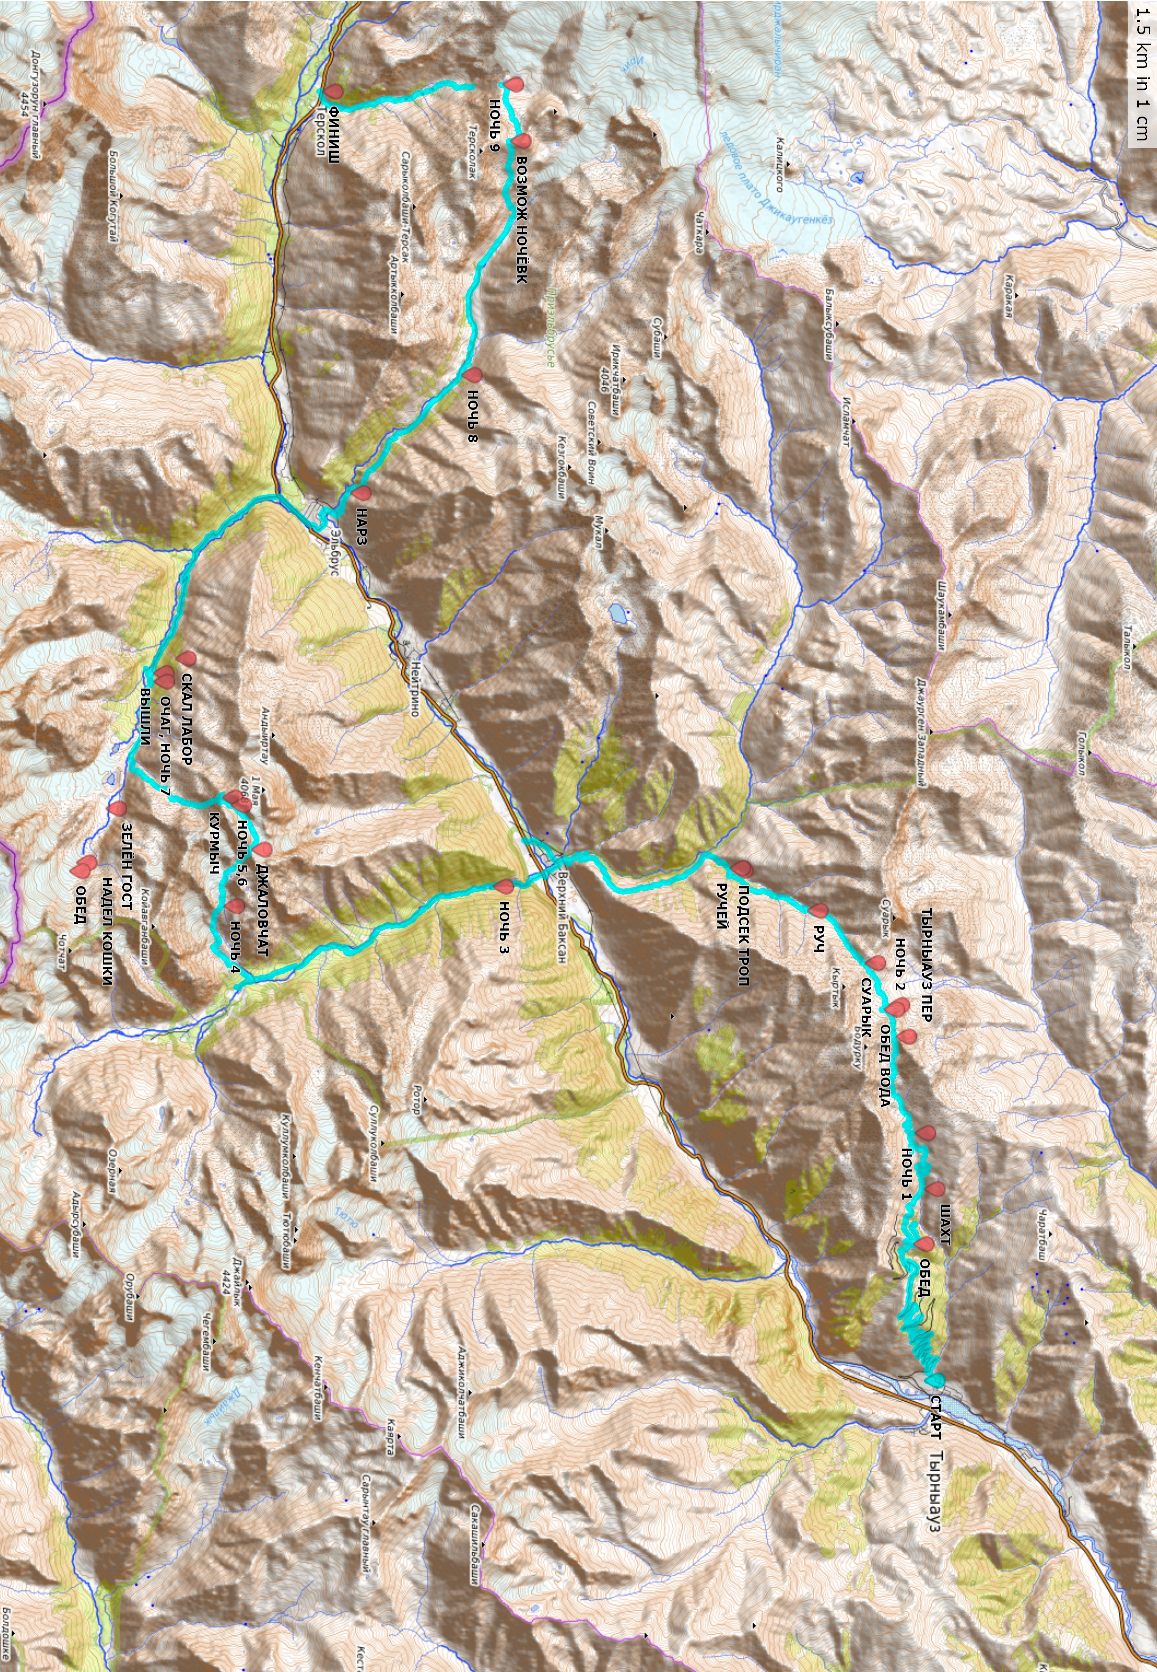
\includegraphics[scale=0.8]{map_all}}
	\caption{Карта пройденного маршрута }
	\label{map_all}
\end{figure}



\subsection{Техническое описание}
	
\subsubsection{День 1}
Сели в заказанное такси в 7.00
Пока доехали, пока разгрузились, было уже 8.00. Пока ехали, было решено немного откорректировать маршрут- пойти не по тропам, а по дороге, и выйти на нужный трек- на горизонте появились облака, а автор отчета, по которому готовился этот участок пути указывал, что под дождем там не очень комфортно идти.

Впрочем, дождя так и не случилось, и за исключением последних ходовых часов, весь день жарило солнце. 
Дорога от тырнауза до верховьев д.р.Тырныауз достаточно широкая, с покрытием типа грунтовка, и весьма не малолюдная- за полдня на ней мы встретили около 5 машин.

Воды в низовьях долины нет совсем, поэтому если группа планирует там пойти- лучше набрать с собой побольше. Через несколько часов пути, примерно в 11.30, мы встретили мужичка травника Володю, который подсказал нам что недалеко есть родник (который указан только на Ляпинке). Перед поворотом на родник мы при сделали привал-обед в 12.00, наиболее бойкая часть команды пошла на разведку, а потом и сходила за водой для всех. 

После обеда мы подрезали планируемый трек, и пошли вдоль всяких разваленных шахт до старой морены, посмотрели на запасной вариант ночевки возле шахт, дружно решили что оно нам не надо, и пошли дальше.

Поднялись по морене, вышли на еще одну грунтовку.
К этому моменту стало чуть прохладнее, идти сталдо приятнее. В этой местности довольно обширная сеть дорог, проложенная шахтерами, но в плохой видимости она только немного путала, нежели чем помогала.
Ручей, который нарисован на картах, мы так и не смогли обнаружить, и долго искали место ночевки. К счастью, один из участников нашел два микроозера (которые тоже указаны на ляпинке, хоть и чуть дальше, чем фактитчески были). Там и заночевали в 19.00. Периодически, когда раздувало облака, мы видели разные дырки в горах- бывшие шахты. которых тут в избытке. Отличнная штука в качестве достопримечательности, особенно если послушать М.В. Расторгуева, который утверждал, что тут в нулевых мужики с автоматами бегали. 

Приятный бонус этой ночевки: виден \tyr и Баксанская долина с необычного ракурса, ловит сеть.

\subsubsection{День 2}
Утром вышли в 8.00, перевал видно, хоть из-за него выглядывают облачка. Движемся сначала по дороге, затем по старым моренам, идут все неплохо, и мы доходим до перевала \tyr в 10.40. На перевале мерзкое облако, совершаем все ритуальные действия (записка-фотка-шоколад), и бегом уходим оттуда. С подьемной стороны перевал не представляет никакой сложности даже в плохую погоду. Со спусковой- в целом тоже, но одна девочка все равно идет  неуверенно.
Спуск с перевала представляет собой мелкую осыпь с чуть видной тропой. В 12.10 спускаемся на зеленые поляны рядом с ручьем, обедаем. Пока идет обед,замечаю, что наш следующий перевал на сегодня окутан недружелюбным облаком, которое скоро припозает нам. Облако начинает протекать, мы ставим тенты палаток и сидим так час. Дальше становится ясно, что сегодня мы не пойдем перевал - с него все еще тянет дождевое облако, а в описании четко указано- в дождь это гадость полная. Поэтому мы переносим палатки на площадки в 50 метрах ниже, и встаем на ночевку в 16.00. Ночеки неплохие- есть подобие ветрозащитных стенок, вода недалеко.

\subsubsection{День 3}
Вышли с ночевки в сторону пер.Суарык  7.00, начали движение по моренам, затем вышли на приятную траву. На перевал Суарыкк вышли в 8.15. По мнению автора этого отчета, на пер.Суарык подниматься в дождь также опасно, как на любой травяой перевал 1А.
На перевале красивый вид, видно и Эльбрус, и наш предстоящий перевал Джаловчат.
Спуск с перевала начинается с едва заметной тропы по мелкой сыпухе, периодически тропа пропадает. 

В итоге мы попали в приятную зеленую долину, и к сожалению, сбились с тропы, поэтому далее просто траверсировали склоны  слева ручья ПХД держась примерно трека, но на 50м выше.
Мы шли то по травяным полям, то по козьим тропам, то форсировали приятный хвойный лес. Когда мы оказались над местом где надо переходить реку, начали спускаться вниз, и все таки увидели тропу.
Перешли ручей, и начали двигаться по правому борту ручья ПХД. 

Вышли в д.р. Кыртык на знакомую дорогу. За пару часов добежали до Верхнего Баксана (вышли в 13.30), где у нас  была заброска. К сожалению, из-за некоторого недопонимания между руководителем и ответственным за заброску, сделали лишний крюк.

После потрошения заброски пошли в долину Адырсу прихватив с собой пса Месснера. 
Долина Адырсу хорошо хожена, поэтому в тщательном описании не нуждается. 
В 17.00 дошли до пограничников, после соблюдения всех формальностей встали на ночевке сразу за ними- на хорошо оборудованной площадке.

К этому моменту мы отставали от графика на 1-2 перехода.


\subsubsection{День 4}	
В этот день нам предстоял подъем до ночевок под пер.Джаловчат. Двигались от м.н. до д.р.Джаловчат по хорошей дороге. Далее двигались по набитой тропе в д.р.Джаловчат. Преодолев несколько ступеней,  В 13.30 пришли на хорошие ночевки в бывшем озере, не дойдя до планируемых 1 переход. Жаркое солнце немного вымотала людей, поэтому решили встать на ночевке прямо тут.


\subsubsection{День 5}
Вышли с ночевки в 6.35, и начали двигаться слегка забирая вправо вверх ПХД по старой морене ледника. За 40 минут дошли до планируемого места ночевки. Там становится ясно, что год очень малоснежный- снежник, который обычно идет до большого камня перед подьемом на Джаловчат почти весь вытаял. Далее идем плотной группой. За 1 маленький переход доходим до начала основного подьема на Джаловчат. После отдыха начинаем подниматься выше по некрутым скалам, выбирая наиболее безопасный путь. Спустя 20 минут движения выходим на турики, впрочем, быстро их теряем, и двигаясь по курумнику, доходим до пер.Джаловчат.


Начинаем надевать системы и кошки, вешаем одну полную веревку вниз. На леднике Курмычи снега почти нет, а там где он есть, он очень не глубокий. Дюльферяем вниз по очереди, после дюльфера все идут на личной технике вниз до небольшого островка с камнями, где мы и собираемся. Снежная обстановка позволяет не связываться. 
Последним уходит Чаплыгин, и выманивает за собой собаку- та отказалась ввязываться в импровизированную систему, и бегала на вольном выпасе.
В итоге героический пес спустился на личной технике, и довольный убежал к основной части команды.
Всего дюльфер занял 2 часа. 

Далее за 40 минут дошли до планируемого места ночевки нагнав график. Сначала шли по открытому леднику, затем по камушкам и снегу. Ночевали в уютном кармане под перевалом. 

\subsubsection{День 6}
Утром проснулись в 4.00, увидели что на улице очень плохая погода. и решили отложить подьем до 8.00. Чуда не случилось, в итоге мы отсиживались весь день, то играя в 'Нечто', то сжигая всякие горелки.

\subsubsection{День 7}
Опять встаем в 4 утра, погода хороша, ппоэтому начинаем собираться. В 6.20 выходим, идем по средней и крупной сыпухе,  в 6.42 приходим на пер.Курмычи. Одну девочку горнит, помимо этого вся группа была уставшей после внезапной 'дневки', и мы решаем пойти запасным путем, минуя вершины сразу вниз.

Спускались по мелкой осыпи, которая сначала была приятно подморожена. Шли плотнй группой, сыпоха хоть и мелкая, но когда начинает ехать, тащит средние камни. Кажется что есть тропа, но возможно это плод фантазий. В итоге в 9 часов доходим до травы, и дальше идем по знакомой тропе. Спуск вниз сложностей не представляет, и в 11 часов мы выходим к началу прижимов в долине Адылсу. Там приваливаемся, и дальше парами доходим до поста пограничников- несмотря на индивидуальные пропуска, выпускать людей без руководителя дежурный отказался.

В 12.00 мы были в лагере Джантуган. Поляна рядом с очагом забита полностью, поэтому ночуем на левой стороне реки (орогр.).



\subsection{Снаряжение, продукты, аптека}

\subsection{Выводы и рекомендации}

	
\end{document}